\documentclass[sutton_barto_notes.tex]{subfiles}
\begin{document}

\newpage
\section{On-policy Control with Approximation}

In this chapter we move from prediction problem to control problem, now with parametric approximation of the action-value $\hat{q}(s,a,\bm{w})\approx q_*(s,a)$.

We learn the semi-gradient SARSA algorithm as the natural extension of semi-gradient TD(0) to action values and to on-policy control.

Once we have genuine function approximation we have to give up discounting and switch to a new `average-reward' formulation of the control problem, with new `differential' (just difference) value functions.

\subsection{Episodic Semi-gradient Control}

From chap 9 $S_t -> U_t$ to chap 10 $S_t, A_t -> U_t$

The general GD update for action-value prediction is
$$\bm{w}_{t+1} \doteq \bm{w}_t + \alpha[U_t - \hat{q}(S_t, A_t, \bm{w}_t)]\nabla \hat{q}(S_t, A_t, \bm{w}_t)$$
Episodic semi-gradient one-step SARSA:
$$\bm{w}_{t+1} \doteq \bm{w}_t + \alpha[R_{t} + \gamma\hat{q}(S_{t+1}, A_{t+1}, \bm{w}_t) - \hat{q}(S_t, A_t, \bm{w}_t)]\nabla\hat{q}(S_t, A_t, \bm{w}_t)$$

\subsection{Semi-gradient n-step SARSA}
\subsection{Average Reward: A New Problem Setting for Continuing Tasks}
Episodic, discounted, average reward (New!)

\paragraph{why average reward} In discounted setting, the only way to ensure the agents actions maximize reward over time is to keep increasing discount factor $\gamma$ towards 1 (see the LeftRight8ring example). The $\gamma$ can't be 1; otherwise, the return will be infinite. Moreover, larger $\gamma$ can result in larger and more variables sums (longer time horizon $\to$ larger discount factor $\to$ wider the range of return $\to$ larger variance), which might be hard to learn. So we introduce a new setting: average reward.

\begin{definition}
\textbf{average reward $r(\pi)$}, no discounting considered, the agent cares the same for delayed rewards and immediate rewards. It defines the quality of a policy $\pi$.
\end{definition}
\begin{align*}
r(\pi)&\doteq \lim_{h\to\infty} \frac{1}{h} \sum_{t=1}^h \E[R_t|S_0, A_{0:t-1} \sim \pi]\\
&=\lim_{t\to\infty}\E[R_t|S_0, A_{0:t-1} \sim \pi]\\
&=\sum_s \mu_\pi(s) \sum_a \pi(a|s) \sum_{s',r} p(s',r|s,a)r
\end{align*}
Note that the expectation conditioned on initial state $S_0$ and all actions according to $\pi$. The 2nd and 3rd equations hold if the MDP is \textbf{\textit{ergodic}}, that is, the \textit{steady-state distribution} $\mu_\pi(s)\doteq lim_{t\rightarrow\inf}P{S_t=s|A_{0:t-1}\sim\pi}$ exists and is independent of $S_0$.
In other words, in the long run, the expectation f being in a state depends only on the policy and the MDP transition probabilities (the effect of early decisions is temporary).

The steady state distribution $\mu_\pi$ is the special distribution under which you remain in the same distribution if you select actions according to $\pi$.

We consider all policies that attain the maximal value of $r(\pi)$ to be optimal.

\begin{definition}
\textbf{differential return}, diff return.
$$G_t \doteq R_{t+1} - r(\pi) + R_{t+2} - r(\pi) + ...$$
\end{definition}
\begin{itemize}
\item The differential return can only be used to compare actions if the same policy is followed on subsequent timesteps.
\item we use average reward to compare policies.
\item Only true $r(\pi)$ results in convergence
\end{itemize}

Bellman equations for differential value functions:
\begin{align*}
v_\pi(s) &= \sum_a \pi(a|s)\sum_{r,s'}p(s',r|s,a)[r-r(\pi)+v_\pi(s')]\\
q_\pi(s,a)&=\sum_{r,s'}p(s',r|s,a)[r-r(\pi)+\sum_{a'}\pi(a'|s')q_\pi(s',a')]\\
v_*(s)&= max_a \sum{r,s'}p(s',r|s,a)[r-max_\pi r(\pi) + v_*(s')]\\
q_*(s,a) &= \sum_{r,s'}p(s',r|s,a)[r-max_\pi r(\pi) + max_{a'} q_*(s',a')]
\end{align*}

\subsection{Learning Objectives (UA RL MOOC)}
Lesson 1: Episodic Sarsa with Function Approximation 

1. Explain the update for Episodic Sarsa with function approximation 
$$\bm{w}_{t+1} \doteq \bm{w}_t + \alpha[R_{t} + \gamma\hat{q}(S_{t+1}, A_{t+1}, \bm{w}_t) - \hat{q}(S_t, A_t, \bm{w}_t)]\nabla\hat{q}(S_t, A_t, \bm{w}_t)$$

2. Introduce the feature choices, including passing actions to features or stacking state features 

\begin{figure}[h!]
  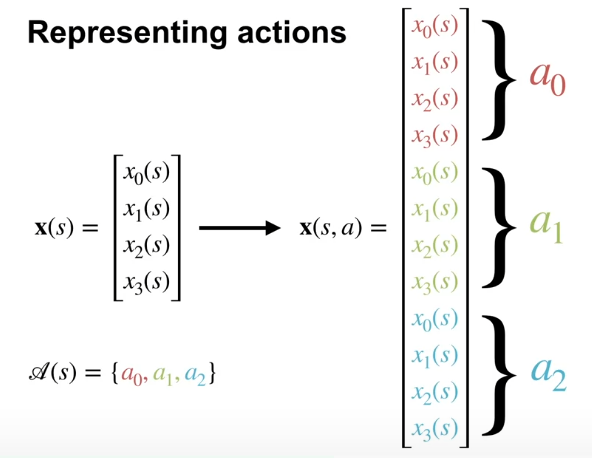
\includegraphics[width=0.5\linewidth]{chap10_feature_stacking.png}
  \caption{feature stacking}
  \label{fig:feature-stacking}
\end{figure}

3. Visualize value function and learning curves 

4. Discuss how this extends to Q-learning easily, since it is a subset of Expected Sarsa 

Expected SARSA:
$$\bm{w}_{t+1} \doteq \bm{w}_t + \alpha[R_{t} + \gamma\sum_{a'}\pi(a'|S_{t+1})\hat{q}(S_{t+1}, A_{t+1}, \bm{w}_t) - \hat{q}(S_t, A_t, \bm{w}_t)]\nabla\hat{q}(S_t, A_t, \bm{w}_t)$$
Q-learning:
$$\bm{w}_{t+1} \doteq \bm{w}_t + \alpha[R_{t} + \gamma max_{a'}\hat{q}(S_{t+1}, A_{t+1}, \bm{w}_t) - \hat{q}(S_t, A_t, \bm{w}_t)]\nabla\hat{q}(S_t, A_t, \bm{w}_t)$$

Lesson 2: Exploration under Function Approximation 

5. Understanding optimistically initializing your value function as a form of exploration

Recall Optimistic Initial values in the tabular setting to encourage early exploration. Note that it's unclear how to optimistically init values with nonlinear function approximators like NN.

Lesson 3: Average Reward 

6. Describe the average reward setting 

Instead of using discount factor, we consider all reward equally.

7. Explain when average reward optimal policies are different from discounted solutions 

Recall the LeftRight8ring example, the optimal policies changes with the choice of $\gamma$. However, the average reward optimal policies gives the same result

8. Understand how differential value functions are different from discounted value functions

Discounted value functions uses discount factor on future rewards, while differential value functions subtract a constant $r(\pi)$ from all rewards.

\end{document}